\documentclass[tikz,border=8pt]{standalone}
\usepackage[T1]{fontenc}
\usepackage{mathpazo}
\usetikzlibrary{arrows.meta, positioning, calc}

\definecolor{stblue}{HTML}{7B97AD}
\definecolor{rwgold}{HTML}{B8995E}
\definecolor{dkbrown}{HTML}{3D3530}
\definecolor{wmgray}{HTML}{7B7067}
\definecolor{cream}{HTML}{F9F6F0}
\definecolor{border}{HTML}{D4C9B8}

\begin{document}
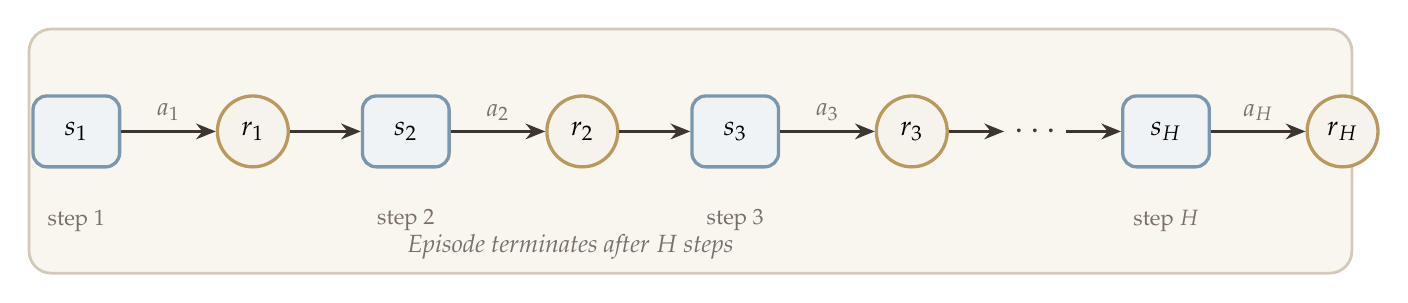
\begin{tikzpicture}[
  state/.style={rectangle, rounded corners=5pt, draw=stblue, line width=1.2pt,
    fill=stblue!12, minimum width=11mm, minimum height=9mm, font=\bfseries},
  reward/.style={circle, draw=rwgold, line width=1.2pt,
    fill=rwgold!12, minimum size=9mm, font=\bfseries},
  >={Stealth[length=2.5mm, width=2mm]},
  arr/.style={draw=dkbrown, line width=0.9pt, ->},
  act/.style={font=\small, text=wmgray, above, midway},
  slab/.style={font=\footnotesize, text=wmgray, below=4mm},
]

% Background
\fill[cream, rounded corners=8pt] (-0.6,-1.8) rectangle (16.2,1.3);
\draw[border, rounded corners=8pt, line width=1pt] (-0.6,-1.8) rectangle (16.2,1.3);

\node[state] (s1) at (0,0) {$s_1$};
\node[reward, right=12mm of s1] (r1) {$r_1$};
\node[state, right=9mm of r1] (s2) {$s_2$};
\node[reward, right=12mm of s2] (r2) {$r_2$};
\node[state, right=9mm of r2] (s3) {$s_3$};
\node[reward, right=12mm of s3] (r3) {$r_3$};
\node[right=7mm of r3, font=\large, text=dkbrown] (dots) {$\cdots$};
\node[state, right=7mm of dots] (sH) {$s_H$};
\node[reward, right=12mm of sH] (rH) {$r_H$};

\draw[arr] (s1) -- node[act] {$a_1$} (r1);
\draw[arr] (r1) -- (s2);
\draw[arr] (s2) -- node[act] {$a_2$} (r2);
\draw[arr] (r2) -- (s3);
\draw[arr] (s3) -- node[act] {$a_3$} (r3);
\draw[arr] (r3) -- (dots);
\draw[arr] (dots) -- (sH);
\draw[arr] (sH) -- node[act] {$a_H$} (rH);

\node[slab] at (s1.south) {step 1};
\node[slab] at (s2.south) {step 2};
\node[slab] at (s3.south) {step 3};
\node[slab] at (sH.south) {step $H$};

\node[font=\small\itshape, text=wmgray]
  at ($(s2.south)!0.5!(s3.south) + (0,-10mm)$)
  {Episode terminates after $H$ steps};
\end{tikzpicture}
\end{document}
